\documentclass[onecolumn,showpacs,pre,preprintnumbers,floatfix]{revtex4-1}
\usepackage{graphicx}
\usepackage[english]{babel}
\usepackage{amssymb}
\usepackage{amsbsy}
\usepackage{amsmath}
\usepackage{color}
\usepackage{natbib}
\graphicspath{/Users/camalupente/Desktop/MIT/Austin_collaboration_3D_flow_George_Brios/manuscript/images/}


\newcommand{\bigO}{\mathcal{O}}
\newcommand{\DD}{\mathcal{D}}
\newcommand{\ff}{\mathbf{f}}
\newcommand{\nn}{\mathbf{n}}
\newcommand{\rr}{\mathbf{r}}
\renewcommand{\SS}{\mathcal{S}}
\newcommand{\ssigma}{\boldsymbol{\sigma}}
\newcommand{\todo}[1]{\fbox{{\bf TODO:} \color{red} #1}}
\newcommand{\uu}{\mathbf{u}}
\newcommand{\xx}{\mathbf{x}}
\newcommand{\yy}{\mathbf{y}}


\begin{document}

\title{On the origin of velocity distributions: a connection with the medium structure}

\author{Pietro de Anna}
\email[E-mail:]{pietro.deanna@unil.ch}
\affiliation{Institut des sciences de la Terre (ISTE) - UNIL, Lausanne 1015, CH}
\author{Bryan Quaife}
\affiliation{Scientific Computing - Florida State University Tallahassee, FL, US}
\author{George Biros}
\affiliation{Institute for Computational Engineering and Sciences - UT Austin, TX, US}
\author{Ruben Juanes}
\affiliation{Civil and Environmental Engineering - MIT, Cambridge 02139 US}

\begin{abstract}
	abstract
\end{abstract}

\maketitle
This manuscript is a summary of the ideas and results we got in the
past year about our study about the link between the velocity
distribution in porous media and the host medium geometrical
properties. In particular, we seek for the link between the often
observed power laws distribution of low velocities in porous materials
and its geometrical properties. Briefly, we hypothesize that the flow
within a single pore is equivalent to the Poiseuille flow through a
pipe for given effective  pressure gradient and radius. Thus the
distribution of the flow through the entire pore network is assumed to
be equivalent to a collection of Poiseuille flows through pipes of a
given effective pressure gradient and radius distribution.\\

\todo{Introduction to the problem of linking the host medium structure
properties and the resulting fluid velocity distribution. Motivating the
choice of investigating power law distributed pore sizes media.}

In this work we consider a $2D$ porous medium whose solid, impermeable,
grain structure is represented by the gray disks in
Figure~\ref{f:normVelocity}.  A constant density incompressible flow
with volumetric flow rate $Q$, with no-flow boundary conditions at the
top and bottom boundaries, is applied from left to right of the porous
domain. The Reynolds number is defined as $Re = \frac{\lambda
\overline{u}}{\nu}$, where $\lambda = 200 \, \mu$m is the average pore
size and $\nu$ is the kinematic viscosity of the fluid (water). The
average velocity is a priori estimated as $\overline{u} = Q / \Sigma
\sim 20 \, \mu$m/s, where $\Sigma = 0.52$ mm$^2$ is the transverse cross
sectional area of the microfluidics (all the quantities have to be
written in the a-dimensional form with respect to characteristic length
and time scales).
%
\begin{figure}[h!]
  \begin{center}
  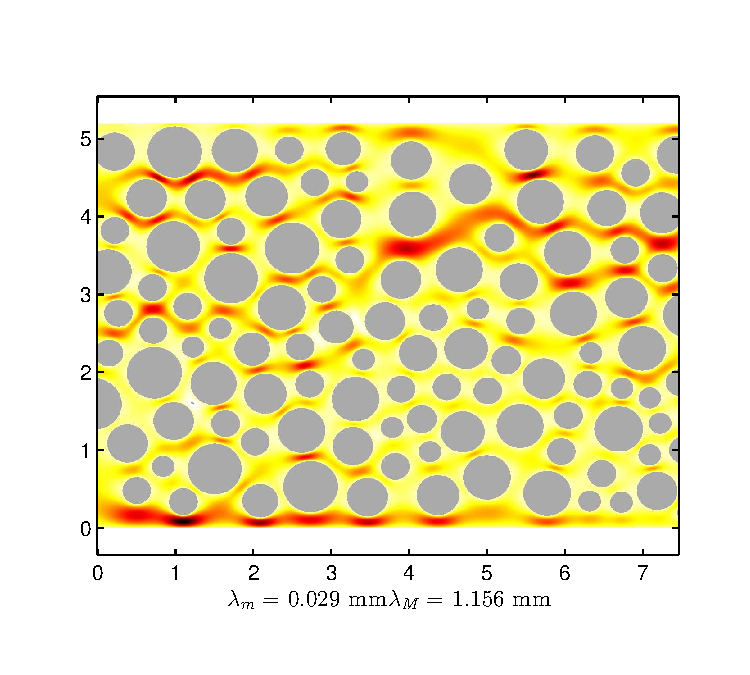
\includegraphics[width=0.49\textwidth]{./images/ux_UT.pdf}
  \caption{The magnitude $|u| = \sqrt{u_x^2 + u_y^2}$ of the flow field
  (Stokes flow) within the considered porous medium, measured with
  P.I.V. \todo{this plot is missing}(left) and simulated (right). The
  minimum and maximum transverse pore sizes are $\lambda_m = 29 \, \mu$m
  and $\lambda_M = 1.15$ mm respectively.}\label{f:normVelocity}
  \end{center}
\end{figure}
%
Thus $Re \sim 0.004$ and the stationary incompressible flow can be approximated by the Stokes flow equations:
%
\begin{align}
  \mu \nabla^2 \boldsymbol{u}(\boldsymbol x) = \nabla p, \quad 
  \nabla \cdot \boldsymbol{u}(\boldsymbol x) = 0.
  \label{e:stokes}
\end{align}
%
Shown in Figure~\ref{f:normVelocity} is the magnitude $|u| = \sqrt{u_x^2
+ u_y^2}$ of the flow which is computed with an integral equation method
\todo{Bryan: describe in later section how this is done}.  The
distribution of the $i^{th}$ velocity component is defined as
%
\begin{align}
  \tilde{p}(v_i) & = & \frac{1}{V} \int_{\Omega} 
  \textrm{d} \boldsymbol x \, 
  \delta\left(v_{i} - \boldsymbol{u}_i(\boldsymbol x)\right) \nonumber \\
  & = &\frac{1}{V} \sum_{j=1}^{n} \int_{\Omega_j} 
  \textrm{d} \boldsymbol x \, 
  \delta\left(v_{i} - \boldsymbol{u}_i(\boldsymbol x)\right)
  \label{e:velocityDistribution}
\end{align}
\todo{$V$ is undefined}
%
where $\Omega_j$ is the $j$-th component of an arbitrary decomposition
of the spatial domain $\Omega$. The normalized distribution
(Probability Density Function) is, then, given by
%
\begin{align*}
  p(v_i) = \frac{\tilde{p}(v_i)}{\int_{\Xi} \textrm{d} v_i \, 
    \tilde{p}(v_i)},
\end{align*}
%
where $\Xi$ is the ensemble space of all the possible velocity values
$\Xi = [u_{min},u_{max}] \subset \mathbb{R}$ between its minimum
$u_{min}$ and maximum $u_{max}$. Shown in Figure~\ref{f:longVelocities}
are the normalized distributions (PDFs) of the longitudinal ($x$)
velocities, which corresponds to eq.~\eqref{e:velocityDistribution},
where the fluid volume $\Omega_i$ is the spatial resolution of the
adopted numerical method.  The goal of this project is to propose a
statistical upscaled model that is able to predict the fluid velocity
distribution and relate it to the pore geometry.
%
\begin{figure}[h!]
  \begin{center}
  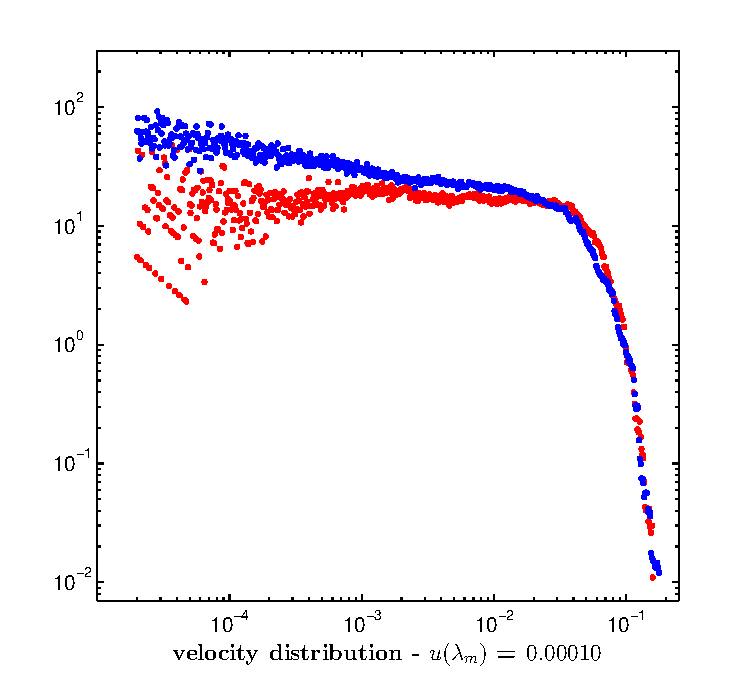
\includegraphics[width=0.49\textwidth]{./images/PDF_ux_loglog.pdf}
  \caption{The normalized distribution (PDF) of the simulated flow
  (blue)\todo{remove the red dots} through the considered pore
  structure.}\label{f:longVelocities}
  \end{center}
\end{figure}
%

\section{The velocity distribution $p(v)$ model}
In order to upscale this system and make predictions on the Stokes flow
distribution in the whole medium, given its geometry, we assume that the
flow in each pore is equivalent to the Poiseuille flow through a pipe of
effective size $L$ and pressure gradient $\nabla p$. The host medium is
a network of pores distributed in size. Thus, we hypothesize that the
global velocity distribution is given by an equivalent, effective,
collection of pipes, distributed in size, in which the flow is driven by
a single effective pressure gradient $\nabla p$.

The spatial profile of the velocity in a pipe in the direction
transverse to the main flow is parabolic (Hagen-Poiseuille flow), which
in $2D$ reads:
%
\begin{align}
  u_{x}(x,y) = \frac{p_{x}}{2\mu} \left(L^2 - y^2 \right),
  \label{e:poiseuille}
  \todo{Not sure why there was a 4 in the deominator}
\end{align}
%
where $y$ represents the transverse direction in the pipe and $y = 0$ is
its middle position and $L$ the radius. For a given pressure gradient,
$u_{max} = \frac{p_{x}L^{2}}{2\mu}$ is the maximum velocity in the pipe.
For simplicity of the notation, we replace $\frac{p_{x}}{2\mu}$ with $A$
in the following.
%
\begin{figure}[h!]
  \begin{center}
  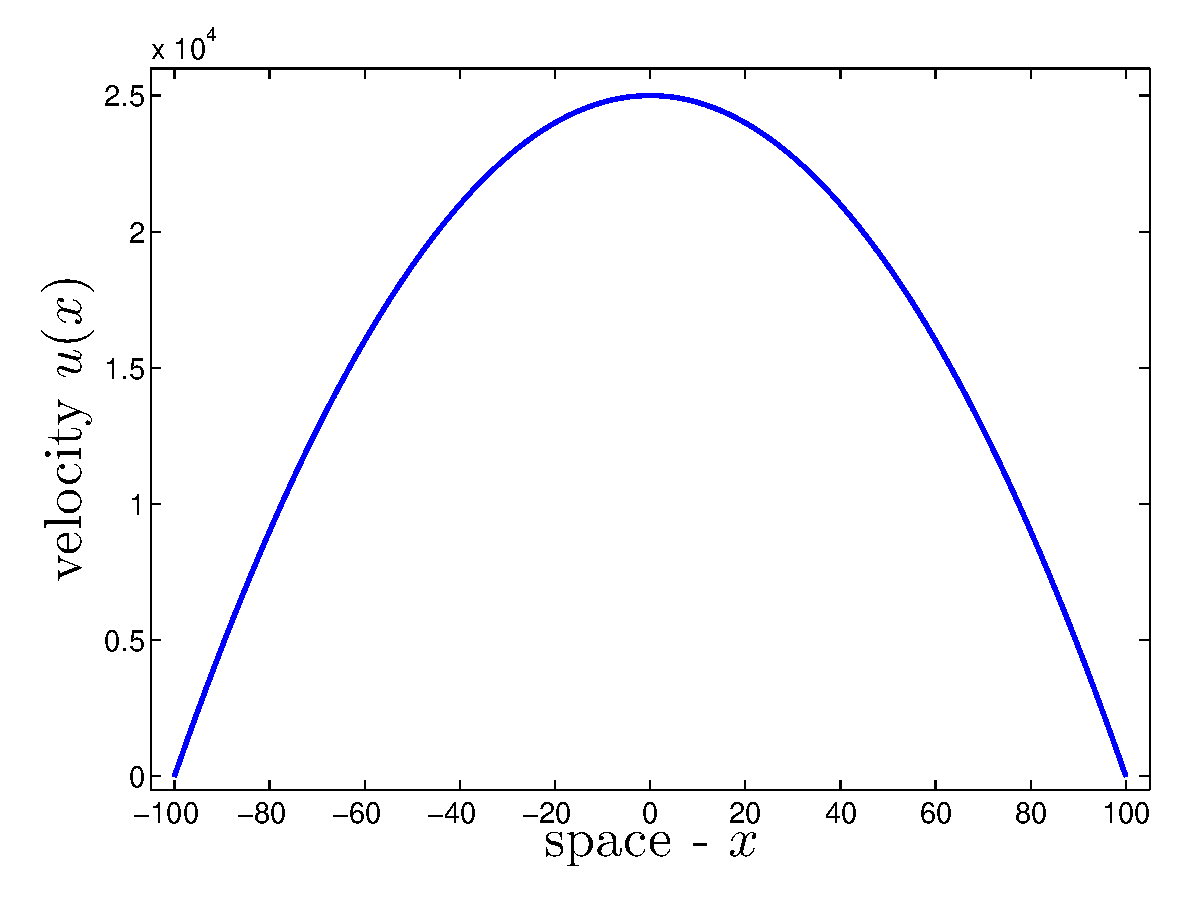
\includegraphics[width=0.49\textwidth]{./images/u.pdf} 
  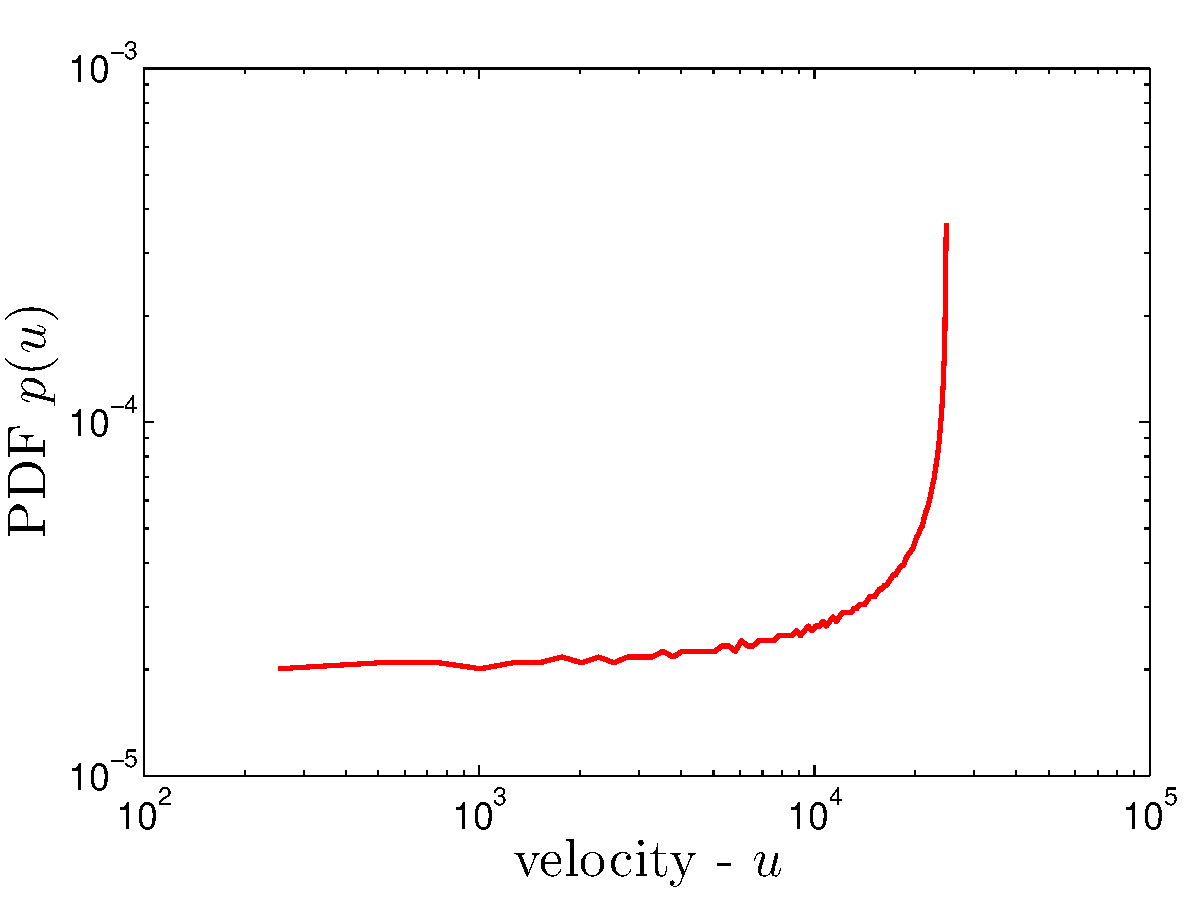
\includegraphics[width=0.49\textwidth]{./images/pdf_u2.pdf}
  \caption{The parabolic profile of the Hagen-Poiseuille flow in a pipe
  of radius.}\label{f:HPflow}
  \end{center}
\end{figure}
%
The distribution $\tilde{p}$ of this parabolic velocity profile is
$\tilde{p}(u) du = \tilde{p}(y) dy$. Since the distribution of a
homogeneous spatial variable $y$ is $1$, we have $\tilde{p}(u) = dy/du$.
We then invert~\eqref{e:poiseuille} obtaining:
%
\begin{align*}
  y(u) = \sqrt{L^2 - \frac{u}{A}}, \quad \Rightarrow \quad 
  \tilde{p}(u) = \frac{dy}{du} = 
  \frac{-1}{2A \sqrt{L^2 - \frac{u}{A}}}.
\end{align*}
\todo{Do we need an absolute value somewhere}
%
Integrating over all the possible velocities:
%
\begin{align*}
  \int_{u_{min}}^{u_{max}} du \, \tilde{p}(u) = \int_{u_{min}}^{u_{max}} 
  du \, \frac{1}{2A \sqrt{L^2 - \frac{u}{A}}} = 
  \left.-\sqrt{L^2 - \frac{u}{A}} \right| _{0}^{AL^2} = L
\end{align*}
%
where $u_{max} = AL^2$ is the velocity in the middle of the channel and
$u_{min} = 0$ is the velocity at the (no-slip) boundary of the pipe.
Thus the normalized velocity distribution is:
%
\begin{align}
  p(u) = \frac1L\frac{dy}{du} = 
    \frac{1}{2AL \sqrt{L^2 - \frac{u}{A}}}
  \label{e:normalizedVelocity}
\end{align}
%

%
\begin{figure}[h!]
  \begin{center}
  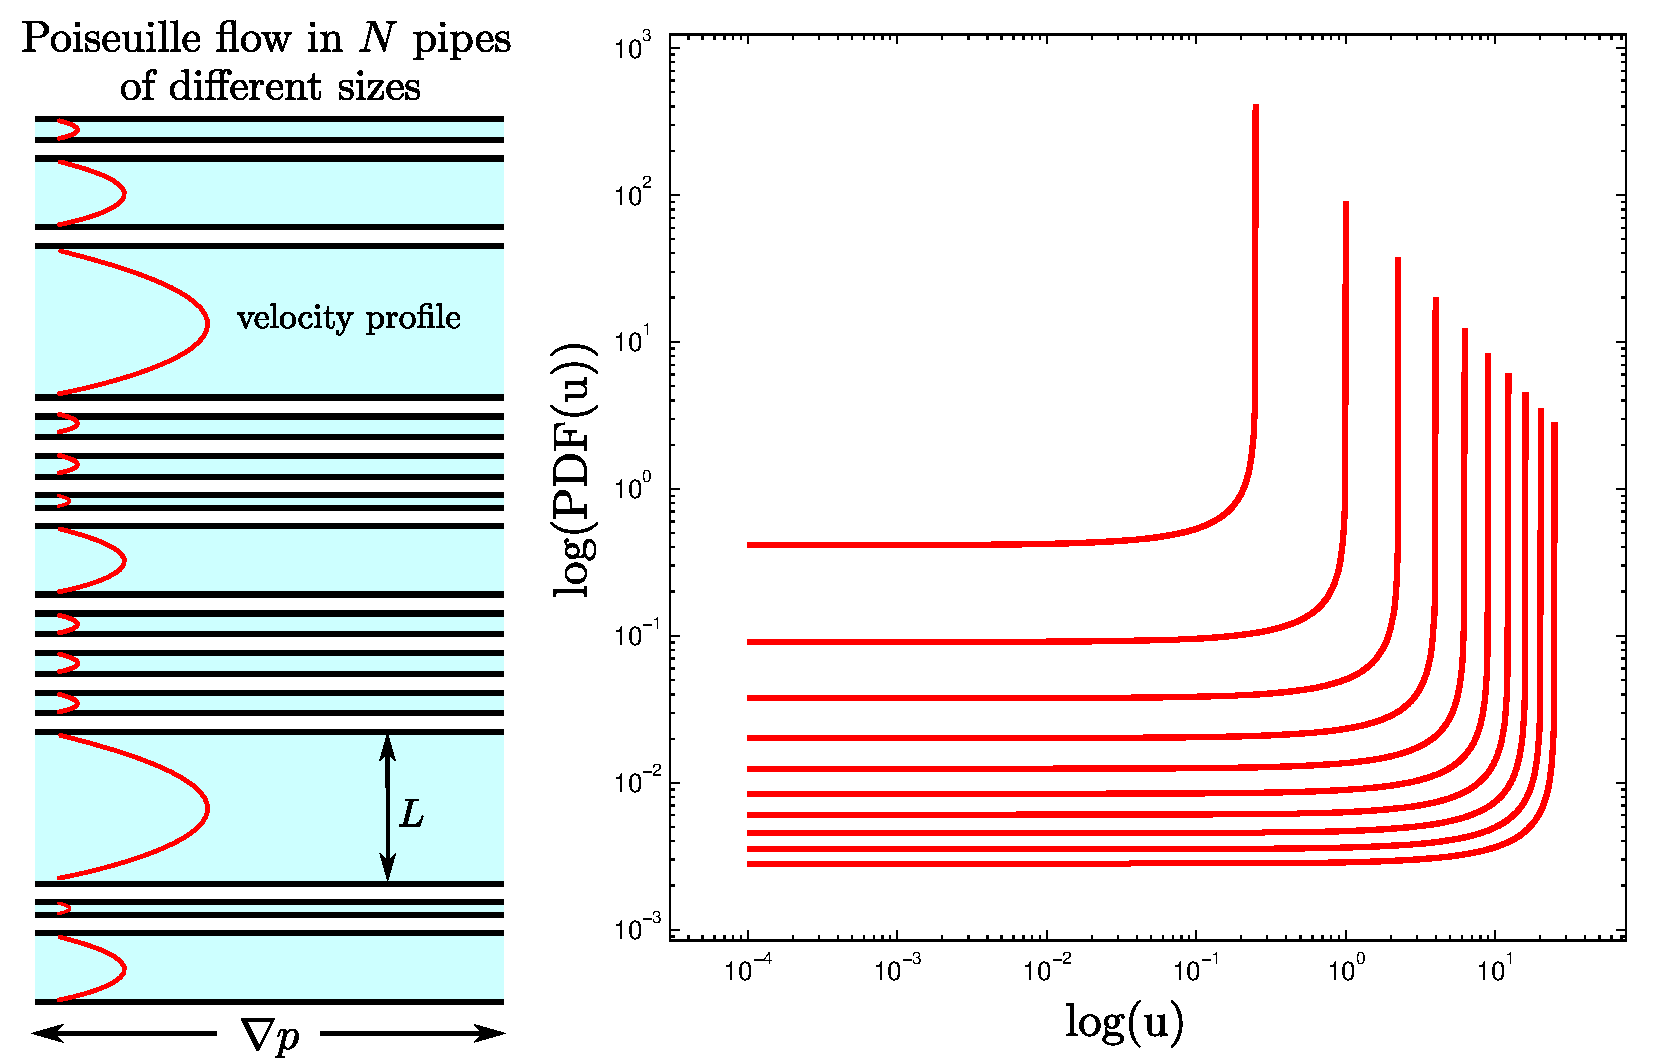
\includegraphics[width=0.49\textwidth]{./images/pipe_scheme.pdf}
  \caption{Left: The parabolic profile of the Hagen-Poiseuille flow in a
  collection of pipes of different radius $L$. Right: The associated
  normalized velocity distribution (PDF).}\label{f:HPflowCollection}
  \end{center}
\end{figure}%
%
%
\begin{figure}[h!]
  \begin{center}
  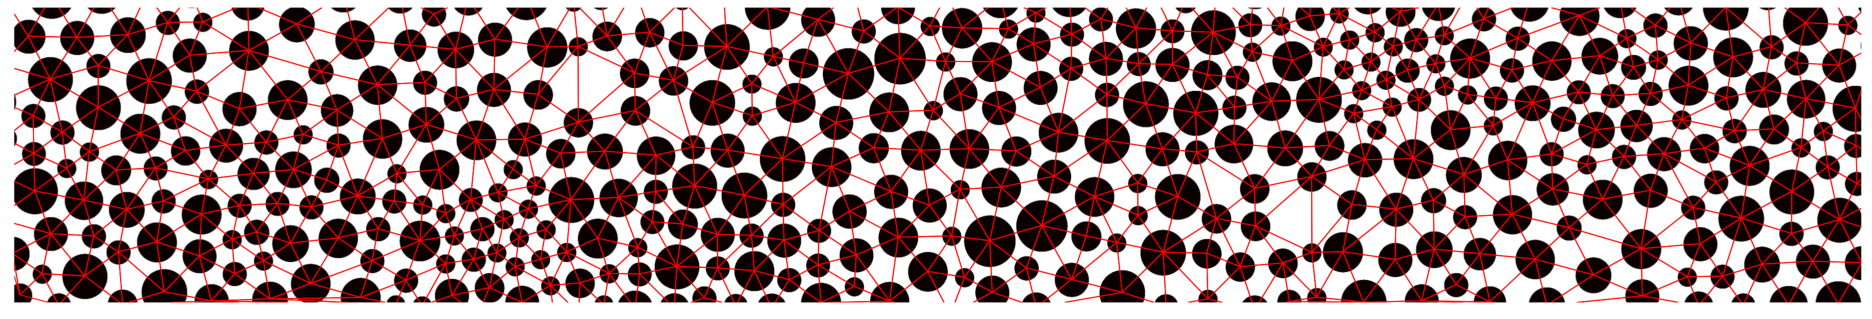
\includegraphics[width=0.49\textwidth]{./images/pore_Delaunay.pdf}
  \caption{Estimation of the transverse pore size
  distribution: length of the segment connecting grains centers using
  Delaunay tessellation.}\label{f:geometryDelaunay}
  \end{center}
\end{figure}
%
The calculated normalized distribution eq.~\eqref{e:normalizedVelocity}
is valid for a given radius $L$.  Now consider a collection of pipes
whose radii are distributed as $p_L(L)$, so that
eq.~\eqref{e:normalizedVelocity} represents the conditional probability
$p_u(u|L)$ distribution, for $L$ given. Thus,
%
\begin{align}
  p(u) = \int_{L(u)}^{L_M} dL \frac{p_L(L)}{\frac{A}{2} 
    \sqrt{L^2 - \frac{u}{A}}}, \quad L(u) = \sqrt{\frac{u}{A}},
  \label{e:collectiveVelocity}
\end{align}
%
where $L(u)$ denotes the radius of a pipe whose maximum velocity is $u$ and $L_M$ the maximum radius according to the distribution $p_L(L)$.\\

Since ... we motivate in the intro the interest of investigating a power
law distributed pore sizes... we now consider that $p_L(L) \sim
L^{-\beta}$, thus, eq.~\eqref{e:collectiveVelocity} becomes
%
\begin{align}
  p(u) & = \int_{L(u)}^{L_M} dL \frac{1}{\frac{\nabla p}{2 \mu}
      L^{\beta} \sqrt{L^2 - \frac{4\mu L}{\nabla p} u}} \nonumber \\ 
    & = 4uL^{-\beta - 2} \sqrt{L\left(L - \frac{4\mu u}
      {\nabla p}\right)} \left( \frac{L \nabla p}{4\mu u} \right)^
      {\beta + 3/2} {}_2F_1\left(\frac12,\beta + \frac12; \frac32; 1 - \frac{L
      \nabla p}{4\mu u}\right) \Bigg|_{L(u)}^{L_M} \nonumber \\
    & = 4L_M^{-\beta - 1} \sqrt{1 - \frac{u}{u_{max}}} \left(
      \frac{u_{max}}{u} \right)^{\beta + 1/2} {}_2F_1\left(
      \frac12,\beta + \frac12; \frac32; 1 - \frac{u_{max}}{u}\right)
    \label{e:powerVelocity}
\end{align}
%
where ${}_2F_1$ denotes the Gaussian Hypergeometric function. If $L =
\frac{4\mu u}{\nabla p}$ eq.~\eqref{e:powerVelocity} is zero. If $L=L_M$
we have
%
\begin{align*}
  p(u) \sim u^{-\beta - \frac12} \, {}_2F_1\left( \frac12,\beta +
  \frac12; \frac32; 1 - \frac{u_{max}}{u}\right).
\end{align*}
%
For velocities $u \ll u_{max}$ the Hypergeometric function scales as
$u^{\frac12}$, so
%
\begin{align*}
  p(u) \sim u^{-\beta}.
\end{align*}
%

Figure~\ref{f:geomDistribution} shows the pore size distribution of 5
porous media $2D$. Figure~\ref{f:velocityDistribution} shows the
probability density function measured of the associated simulated Stokes
flow. They scale as 
%
\begin{align*}
  p(u) \sim u^{-2\beta}.
\end{align*}
%
\todo{Need to understand the factor 2}

%
\begin{figure}[h!]
  \begin{center}
  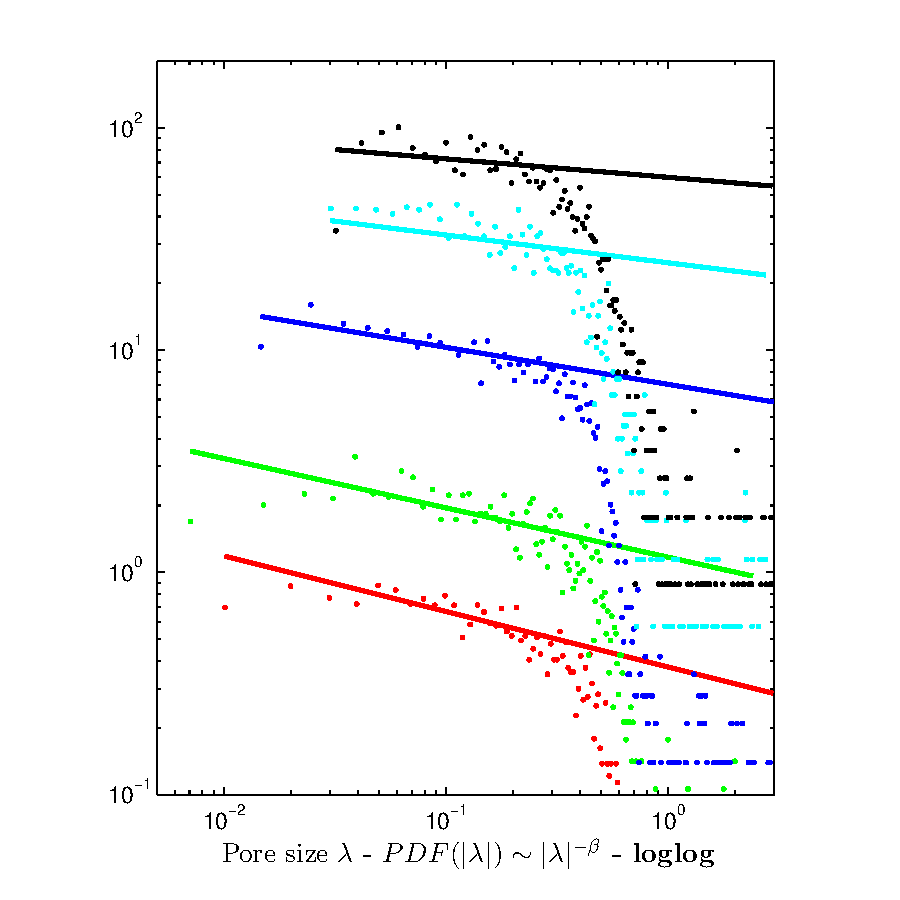
\includegraphics[width=0.49\textwidth]{./images/PDF_all_lambda_shifted.pdf}
  \caption{The pore size $\lambda$ distribution $p(\lambda) \sim
  \lambda^{-\beta}$, of the 5 media simulated, defined as length of the
  segment connecting grains centers using Delaunay tessellation. Power
  laws exponent: $\beta = -1/12$ (black), $\beta = -1/8$ cyan, $\beta =
  -1/6$ blue, $\beta = -1/4.5$ green and $\beta = -1/4$
  red.}\label{f:geomDistribution} 
  \end{center}
\end{figure}
%

%
\begin{figure}[h!]
  \begin{center}
  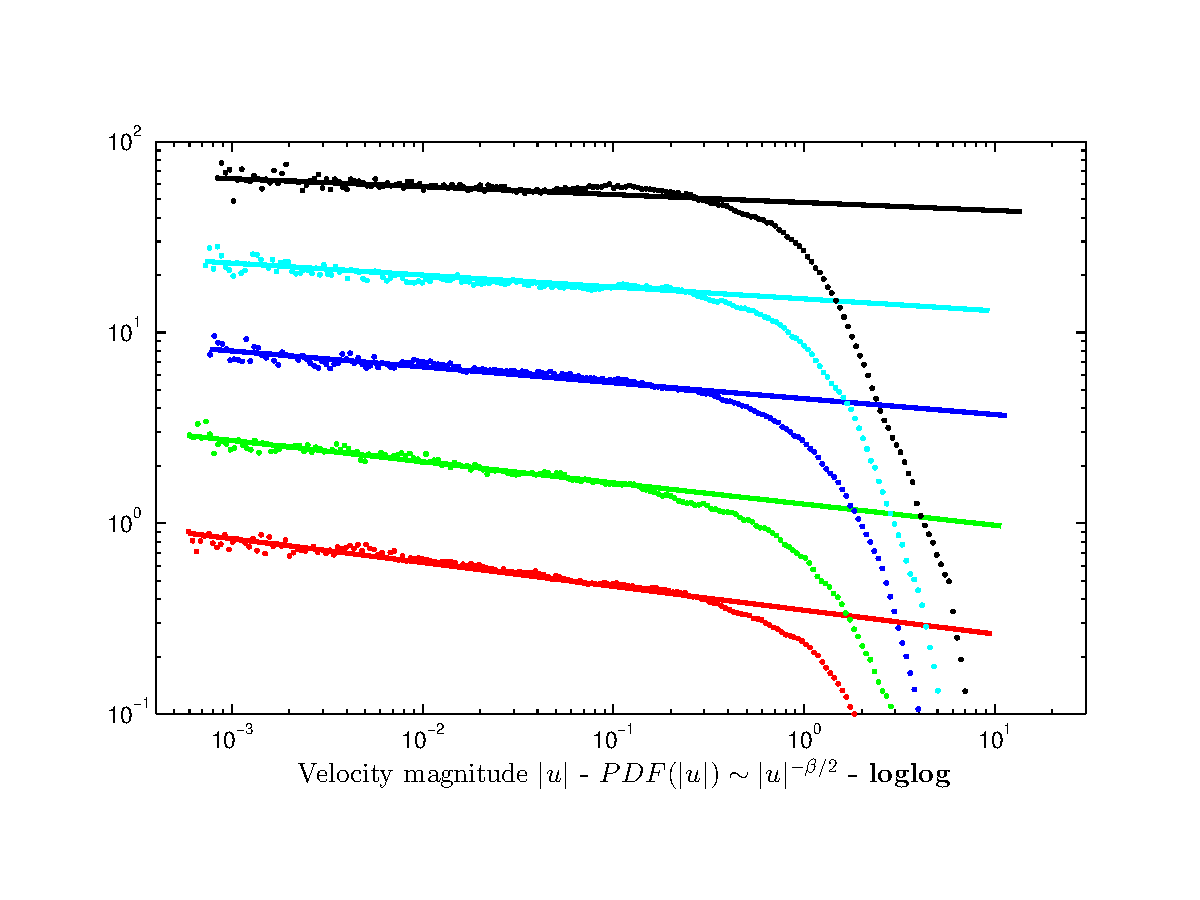
\includegraphics[width=0.49\textwidth]{./images/PDF_all_velo_shifted2.pdf}
  \caption{The velocity $u$ distribution $p(u) \sim u^{-\gamma}$, of the
  5 media simulated, defined as length of the segment connecting grains
  centers using Delaunay tessellation. Power laws exponent $\gamma =
  2\beta$: $\gamma = -1/24$ (black), $\beta = -1/16$ cyan, $\beta =
  -1/12$ blue, $\beta = -1/9$ green and $\beta = -1/8$
  red.}\label{f:velocityDistribution} 
  \end{center}
\end{figure}
%



%%%%%%%%%%%%%%%%%%%%%%%%%%%%%%%%%%%%%%%%%%%%%%%%%%%%%%%%%%%%%%%%%%%%%%%%%
\section{Numerical methods}
Here we describe how the incompressible Stokes equations are
numerically solved in geometries such as the one in
Figure~\ref{f:normVelocity}.  We use an integral equation method since
it naturally resolves the geometry, achieves high-order accuracy,
satisfies the incompressibility constraint with machine precision, and
can be solved in linear time with the fast multipole method (FMM).  Let
the no-slip boundary condition be $\uu = \ff$, and let $\Gamma$ denote
the boundary of the domain $\Omega$.

For any point in the geometry, $\xx \in \Omega \backslash \Gamma$, the
single- and double-layer potentials for the Stokes equations
are~\cite{poz1992}
\begin{align*}
  \SS[\ssigma](\xx) &= \frac{1}{4\pi\mu}\int_{\Gamma} \left(
  -\log\rho I + \frac{\rr \otimes\rr}{\rho^{2}} 
  \right)\ssigma(\yy)ds_{\yy},  \\
  \DD[\ssigma](\xx) &= \frac{1}{\pi}\int_{\Gamma} 
  \frac{\rr \cdot \nn}{\rho^{2}}\frac{\rr \otimes \rr}{\rho^{2}}
  \ssigma(\yy)ds_{\yy},
\end{align*}
where $\rr = \xx - \yy$, $\rho = \|\rr\|$, $\nn$ is the unit outward
normal of $\Gamma$, and $\ssigma$ is referred to as a density
function.  We represent $\uu$ as the combination of single- and
double-layer potentials
\begin{align}
  \uu(\xx) = \sum_{k=1}^{M} \SS[\ssigma_{k}](\xx) + 
    \DD[\ssigma_{0}](\xx).
  \label{e:integralRep}
\end{align}
The no-slip boundary condition is satisfied by solving for $\ssigma$ in
the integral equation defined only on $\Gamma$
\begin{align}
  \ff(\xx_{0}) = \uu(\xx_{0}) + \frac{1}{2}\left\{
    \begin{array}{cl}
      \ssigma(\xx_{0}) & \xx_{0} \in \Gamma_{0}, \\
      0 & \xx_{0} \in \Gamma \backslash \Gamma_{0}.
    \end{array}
    \right. 
    \label{e:integralEqn}
\end{align}
Solutions of~\eqref{e:integralEqn} are guaranteed to exist whenever the
no flux condition $\int_{\Gamma} \ff \cdot \nn=0$ is
satisfied~\cite{poz1992}.

We discretize~\eqref{e:integralEqn} with a Nystr\"{o}m method.  The
density function is discretized at a set of collocation points, and the
integrals are approximated with suitable quadrature rules.  $\SS$ is
discretized with a high-order Gauss-Trapezoid rule~\cite{alp1999}, and,
since the kernel of $\DD$ is smooth, the trapezoid rule, which
converges super-algebraically~\cite{tre:wei2014}, is used to discretize
$\DD$.  The resulting linear system is solved iteratively with
GMRES~\cite{saa:sch1986}, and the matrix-vector multiplication is
computed with $\bigO(N)$ operations by using the FMM~\cite{cmcl2012}.
We use a block-diagonal preconditioner, where each $\Gamma_{k}$,
$k=0,\ldots,M$, corresponds to a block.  For the circle boundaries, the
single-layer potential is known analytically and can be applied
efficiently with $\bigO(N \log N)$ operations with the Fast Fourier
Transform (FFT).  The double-layer potential for the exterior boundary
is precomputed and factorized, but this is manageable since we only use
$N=2048$ points for the exterior boundary.  Preconditioned GMRES with a
tolerance of $10^{-6}$ solves this system with $\bigO(100)$ iterations.

Once~\eqref{e:integralEqn} is solved, the velocity $\uu$ can be
computed at any point $\xx \in \Omega$ by applying the trapezoid rule
to the representation formula~\eqref{e:integralRep}.  However, the
quality of the quadrature rule degrades as $\xx$ approaches
$\Gamma$~\cite{bar2014,bar:wu:vee2014}.  We use a near-singular
integration strategy, first outlined in~\cite{bir:yin:zor2004}, that
guarantees a uniform quadrature error in all of $\Omega$ without
requiring a significant amount of additional computational work.

\bibliography{refs}


\end{document}
